\documentclass[12pt]{article}
\usepackage{graphicx} % for including figures
\usepackage{placeins} % can force floating figures to appear before a barrier
\usepackage{enumerate} % for lists
\usepackage{listings} % for inserting code
\usepackage{soul,color} % for highlighting text
\usepackage{amsmath}
\usepackage{mathtools}
\usepackage{palatino}
\usepackage{mathpazo}
\usepackage{amsmath}
\usepackage{amssymb}
\usepackage{color}
\usepackage{todonotes}
\usepackage{listings}

\pagestyle{plain}
\lstset{showstringspaces=false, % do not use special symbol for string spaces
breaklines=true, %b
breakatwhitespace=true,
} 


% define the title
\author{Samuel Daulton, Andrew Petschek}
\title{Predicting Chess Membership Lapses}
\begin{document}
% generates the title
\maketitle
\begin{center}
GitHub: https://github.com/apetschek/stat147chess
\end{center}

\newpage
\section*{Introduction}
Given a dataset with information about US Chess members in good standing, we were tasked with modeling the probability that a player's membership would be canceled in the near future.  Each data observation includes many features summarizing a player's membership history and type, as well as a player's recent activity and rankings.  We were provided with 43,436 observations to train a model.  The model was than assessed on a test set with 14,479 observations based on the discrepancy of between the predicted probabilities of a membership lapse and the true value of whether the player's membership lapsed.  The true value is 1 if the membership lapsed and 0 otherwise.  The discrepancy function is given by:
$$d = \frac{1}{n}\sum_{i=1}^{n}\left(y_i\log(\hat{p}_i)+(1-y_i)\log(1-\hat{p}_i)\right)$$
where $n$ is the number of samples in the test set.
\section*{Summary of Final Models}
a summary of the final model(s) that you submitted for prediction along with the associated discrepancy measure (you can report the measure based on the 50\% test data sample rather than the final measure).
\section*{Preprocessing}
The dataset contains missing values for several predictor variables.  To replace these missing values, we computed the mean (over all samples in the training data) of each predictor variable for which at least one value was missing.  We then filled the missing values with the mean of that predictor variable.  In addition, for each predictor variable $x_i$ missing at least one value, we created a new predictor variable indicating whether or not a each observation was originally missing the value for $x_i$.  To make predictions on the test set, each missing value of a predictor variable in the test set was filled with the mean of the predictor variable over all observations in the training set.

After addressing the missing values, we split the original training data into training and validation sets.  We then trained models using the (smaller) training set and made predictions on the validation set to ensure that our models were robust to new data.

\section {Exploratory Data Analysis}
Histograms of the quantitative variables showed at many of the quantitative variables were not very spread out, but rather many observations had similar values for these variables.
  \FloatBarrier
  \begin{figure}[!ht]
    \centering
    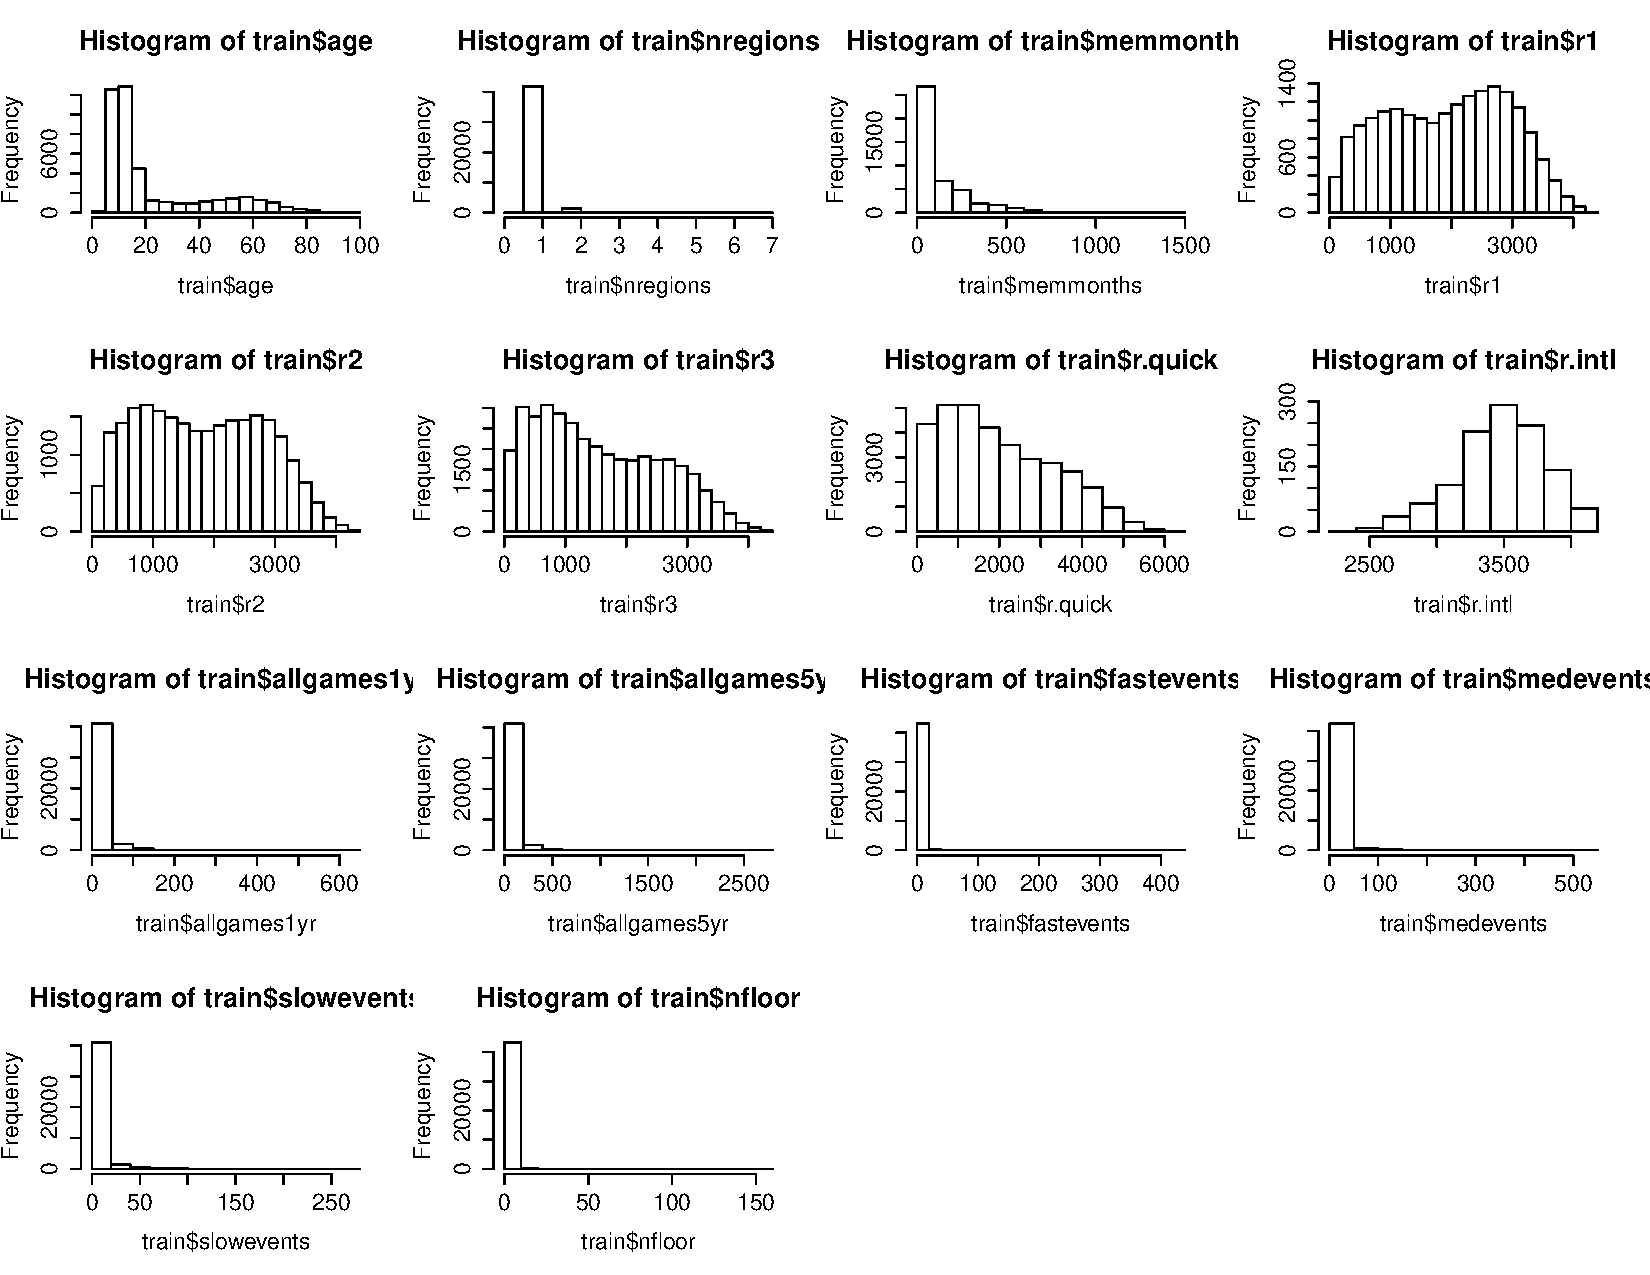
\includegraphics[width=\textwidth]{histograms_of_quant_vars}
    \caption{Scatterplot matrix with all the features in the Auto dataset}
  \end{figure}
  \FloatBarrier
We noted that we may achieve more accurate predictions if we transformed some of these variables (e.g. take the square root) to create more variation between observations.
\section*{Preliminary Models}
Here we outline the sequence of models we built and key insights that led us to change our approach with each model.
\begin{enumerate}
  \item 
  First, we made baseline predictions by fitting a generalized linear model (GLM) using the original features as the predictor variables.  We used likelihood ratio tests to compare the full model to each model with one of the predictor variables removed.  We identified the simpler model that yielded the highest p-value from the Chi-Squared test statistic when compared to the full model in a likelihood ratio test.  This means the the difference between the simpler model and the full model is insignificant, and we choose the simpler model with the highest p-value, meaning least significant difference between simple and complex models.  This simpler model was then used in the subsequent iteration of likelihood ratio tests, comparing it to all models with another feature removed.  This process was continued until all likelihood ratio tests showed that no simpler model was better.  When tested on 50\% of the test set, this model achieved a discrepancy of 0.56834 
  \item
  To improve upon our baseline predictions, we recalled that we had identified a lack of spread in the distribution of many of the quantitative variables.  To spread out the observed values of the variables, we transformed all the quantitative variables by taking the square root of each variable.  In addition, we incorporated pairwise and 3-way interaction terms between the following variables:age, number of regions, and number of months as a member.  Similar to the first, model we simplified the model as much as possible using likelihood ratio tests.  When tested on 50\% of the test set, this model achieved a discrepancy of 0.56529, an improvement of 0.00305 over the first model.
  \item
  Our next idea was to use generalized additive models, where we took the spline of each quantitative variables in an attempt to model nonlinearities.  Again, we simplified the model as much as possible using likelihood ratio tests.  When tested on 50\% of the test set, this model achieved a discrepancy of 0.54760, an improvement of 0.01769 over the previous model. 
\end{enumerate}
\section*{Analysis of Final Models}
\section*{Next Steps}
\end{document}